\documentclass[1p]{elsarticle_modified}
%\bibliographystyle{elsarticle-num}

%\usepackage[colorlinks]{hyperref}
%\usepackage{abbrmath_seonhwa} %\Abb, \Ascr, \Acal ,\Abf, \Afrak
\usepackage{amsfonts}
\usepackage{amssymb}
\usepackage{amsmath}
\usepackage{amsthm}
\usepackage{scalefnt}
\usepackage{amsbsy}
\usepackage{kotex}
\usepackage{caption}
\usepackage{subfig}
\usepackage{color}
\usepackage{graphicx}
\usepackage{xcolor} %% white, black, red, green, blue, cyan, magenta, yellow
\usepackage{float}
\usepackage{setspace}
\usepackage{hyperref}

\usepackage{tikz}
\usetikzlibrary{arrows}

\usepackage{multirow}
\usepackage{array} % fixed length table
\usepackage{hhline}

%%%%%%%%%%%%%%%%%%%%%
\makeatletter
\renewcommand*\env@matrix[1][\arraystretch]{%
	\edef\arraystretch{#1}%
	\hskip -\arraycolsep
	\let\@ifnextchar\new@ifnextchar
	\array{*\c@MaxMatrixCols c}}
\makeatother %https://tex.stackexchange.com/questions/14071/how-can-i-increase-the-line-spacing-in-a-matrix
%%%%%%%%%%%%%%%

\usepackage[normalem]{ulem}

\newcommand{\msout}[1]{\ifmmode\text{\sout{\ensuremath{#1}}}\else\sout{#1}\fi}
%SOURCE: \msout is \stkout macro in https://tex.stackexchange.com/questions/20609/strikeout-in-math-mode

\newcommand{\cancel}[1]{
	\ifmmode
	{\color{red}\msout{#1}}
	\else
	{\color{red}\sout{#1}}
	\fi
}

\newcommand{\add}[1]{
	{\color{blue}\uwave{#1}}
}

\newcommand{\replace}[2]{
	\ifmmode
	{\color{red}\msout{#1}}{\color{blue}\uwave{#2}}
	\else
	{\color{red}\sout{#1}}{\color{blue}\uwave{#2}}
	\fi
}

\newcommand{\Sol}{\mathcal{S}} %segment
\newcommand{\D}{D} %diagram
\newcommand{\A}{\mathcal{A}} %arc


%%%%%%%%%%%%%%%%%%%%%%%%%%%%%5 test

\def\sl{\operatorname{\textup{SL}}(2,\Cbb)}
\def\psl{\operatorname{\textup{PSL}}(2,\Cbb)}
\def\quan{\mkern 1mu \triangleright \mkern 1mu}

\theoremstyle{definition}
\newtheorem{thm}{Theorem}[section]
\newtheorem{prop}[thm]{Proposition}
\newtheorem{lem}[thm]{Lemma}
\newtheorem{ques}[thm]{Question}
\newtheorem{cor}[thm]{Corollary}
\newtheorem{defn}[thm]{Definition}
\newtheorem{exam}[thm]{Example}
\newtheorem{rmk}[thm]{Remark}
\newtheorem{alg}[thm]{Algorithm}

\newcommand{\I}{\sqrt{-1}}
\begin{document}

%\begin{frontmatter}
%
%\title{Boundary parabolic representations of knots up to 8 crossings}
%
%%% Group authors per affiliation:
%\author{Yunhi Cho} 
%\address{Department of Mathematics, University of Seoul, Seoul, Korea}
%\ead{yhcho@uos.ac.kr}
%
%
%\author{Seonhwa Kim} %\fnref{s_kim}}
%\address{Center for Geometry and Physics, Institute for Basic Science, Pohang, 37673, Korea}
%\ead{ryeona17@ibs.re.kr}
%
%\author{Hyuk Kim}
%\address{Department of Mathematical Sciences, Seoul National University, Seoul 08826, Korea}
%\ead{hyukkim@snu.ac.kr}
%
%\author{Seokbeom Yoon}
%\address{Department of Mathematical Sciences, Seoul National University, Seoul, 08826,  Korea}
%\ead{sbyoon15@snu.ac.kr}
%
%\begin{abstract}
%We find all boundary parabolic representation of knots up to 8 crossings.
%
%\end{abstract}
%\begin{keyword}
%    \MSC[2010] 57M25 
%\end{keyword}
%
%\end{frontmatter}

%\linenumbers
%\tableofcontents
%
\newcommand\colored[1]{\textcolor{white}{\rule[-0.35ex]{0.8em}{1.4ex}}\kern-0.8em\color{red} #1}%
%\newcommand\colored[1]{\textcolor{white}{ #1}\kern-2.17ex	\textcolor{white}{ #1}\kern-1.81ex	\textcolor{white}{ #1}\kern-2.15ex\color{red}#1	}

{\Large $\underline{12n_{0744}~(K12n_{0744})}$}

\setlength{\tabcolsep}{10pt}
\renewcommand{\arraystretch}{1.6}
\vspace{1cm}\begin{tabular}{m{100pt}>{\centering\arraybackslash}m{274pt}}
\multirow{5}{120pt}{
	\centering
	\includegraphics[width=112pt]{../../../GIT/diagram.site/Diagrams/png/2833_12n_0744.png}\\
\ \ \ A knot diagram\footnotemark}&
\allowdisplaybreaks
\textbf{Linearized knot diagam} \\
\cline{2-2}
 &
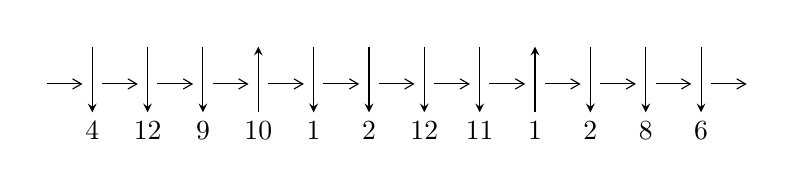
\begin{tikzpicture}[x=20pt, y=17pt]
	% nodes
	\node (C0) at (0, 0) {};
	\node (C1) at (1, 0) {};
	\node (C1U) at (1, +1) {};
	\node (C1D) at (1, -1) {4};

	\node (C2) at (2, 0) {};
	\node (C2U) at (2, +1) {};
	\node (C2D) at (2, -1) {12};

	\node (C3) at (3, 0) {};
	\node (C3U) at (3, +1) {};
	\node (C3D) at (3, -1) {9};

	\node (C4) at (4, 0) {};
	\node (C4U) at (4, +1) {};
	\node (C4D) at (4, -1) {10};

	\node (C5) at (5, 0) {};
	\node (C5U) at (5, +1) {};
	\node (C5D) at (5, -1) {1};

	\node (C6) at (6, 0) {};
	\node (C6U) at (6, +1) {};
	\node (C6D) at (6, -1) {2};

	\node (C7) at (7, 0) {};
	\node (C7U) at (7, +1) {};
	\node (C7D) at (7, -1) {12};

	\node (C8) at (8, 0) {};
	\node (C8U) at (8, +1) {};
	\node (C8D) at (8, -1) {11};

	\node (C9) at (9, 0) {};
	\node (C9U) at (9, +1) {};
	\node (C9D) at (9, -1) {1};

	\node (C10) at (10, 0) {};
	\node (C10U) at (10, +1) {};
	\node (C10D) at (10, -1) {2};

	\node (C11) at (11, 0) {};
	\node (C11U) at (11, +1) {};
	\node (C11D) at (11, -1) {8};

	\node (C12) at (12, 0) {};
	\node (C12U) at (12, +1) {};
	\node (C12D) at (12, -1) {6};
	\node (C13) at (13, 0) {};

	% arrows
	\draw[->,>={angle 60}]
	(C0) edge (C1) (C1) edge (C2) (C2) edge (C3) (C3) edge (C4) (C4) edge (C5) (C5) edge (C6) (C6) edge (C7) (C7) edge (C8) (C8) edge (C9) (C9) edge (C10) (C10) edge (C11) (C11) edge (C12) (C12) edge (C13) ;	\draw[->,>=stealth]
	(C1U) edge (C1D) (C2U) edge (C2D) (C3U) edge (C3D) (C4D) edge (C4U) (C5U) edge (C5D) (C6U) edge (C6D) (C7U) edge (C7D) (C8U) edge (C8D) (C9D) edge (C9U) (C10U) edge (C10D) (C11U) edge (C11D) (C12U) edge (C12D) ;
	\end{tikzpicture} \\
\hhline{~~} \\& 
\textbf{Solving Sequence} \\ \cline{2-2} 
 &
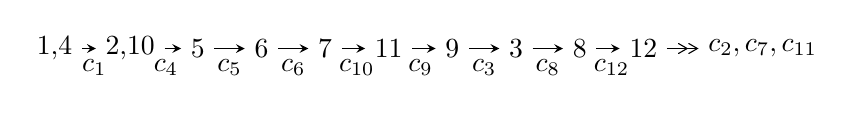
\begin{tikzpicture}[x=23pt, y=7pt]
	% node
	\node (A0) at (-1/8, 0) {1,4};
	\node (A1) at (17/16, 0) {2,10};
	\node (A2) at (17/8, 0) {5};
	\node (A3) at (25/8, 0) {6};
	\node (A4) at (33/8, 0) {7};
	\node (A5) at (41/8, 0) {11};
	\node (A6) at (49/8, 0) {9};
	\node (A7) at (57/8, 0) {3};
	\node (A8) at (65/8, 0) {8};
	\node (A9) at (73/8, 0) {12};
	\node (C1) at (1/2, -1) {$c_{1}$};
	\node (C2) at (13/8, -1) {$c_{4}$};
	\node (C3) at (21/8, -1) {$c_{5}$};
	\node (C4) at (29/8, -1) {$c_{6}$};
	\node (C5) at (37/8, -1) {$c_{10}$};
	\node (C6) at (45/8, -1) {$c_{9}$};
	\node (C7) at (53/8, -1) {$c_{3}$};
	\node (C8) at (61/8, -1) {$c_{8}$};
	\node (C9) at (69/8, -1) {$c_{12}$};
	\node (A10) at (11, 0) {$c_{2},c_{7},c_{11}$};

	% edge
	\draw[->,>=stealth]	
	(A0) edge (A1) (A1) edge (A2) (A2) edge (A3) (A3) edge (A4) (A4) edge (A5) (A5) edge (A6) (A6) edge (A7) (A7) edge (A8) (A8) edge (A9) ;
	\draw[->>,>={angle 60}]	
	(A9) edge (A10);
\end{tikzpicture} \\ 

\end{tabular} \\

\footnotetext{
The image of knot diagram is generated by the software ``\textbf{Draw programme}" developed by Andrew Bartholomew(\url{http://www.layer8.co.uk/maths/draw/index.htm\#Running-draw}), where we modified some parts for our purpose(\url{https://github.com/CATsTAILs/LinksPainter}).
}\phantom \\ \newline 
\centering \textbf{Ideals for irreducible components\footnotemark of $X_{\text{par}}$} 
 
\begin{align*}
I^u_{1}&=\langle 
-170628010722 u^{28}-1866088423702 u^{27}+\cdots+214215715127 b+903136739857,\\
\phantom{I^u_{1}}&\phantom{= \langle  }-903136739857 u^{28}-9593248116983 u^{27}+\cdots+428431430254 a+3314728870309,\\
\phantom{I^u_{1}}&\phantom{= \langle  }u^{29}+11 u^{28}+\cdots-9 u-2\rangle \\
I^u_{2}&=\langle 
- u^{10}+5 u^9-13 u^8+20 u^7-20 u^6+11 u^5- u^4-4 u^3- a u+u^2+b+u-1,\;- u^{10} a- u^{10}+\cdots- a+3,\\
\phantom{I^u_{2}}&\phantom{= \langle  }u^{11}-5 u^{10}+12 u^9-15 u^8+8 u^7+4 u^6-8 u^5+3 u^4+3 u^3-3 u^2+1\rangle \\
I^u_{3}&=\langle 
u^{15}-6 u^{14}+\cdots+b+1,\;- u^{16}+8 u^{15}+\cdots+a+1,\;u^{17}-8 u^{16}+\cdots-5 u^2+1\rangle \\
\\
\end{align*}
\raggedright * 3 irreducible components of $\dim_{\mathbb{C}}=0$, with total 68 representations.\\
\footnotetext{All coefficients of polynomials are rational numbers. But the coefficients are sometimes approximated in decimal forms when there is not enough margin.}
\newpage
\renewcommand{\arraystretch}{1}
\centering \section*{I. $I^u_{1}= \langle -1.71\times10^{11} u^{28}-1.87\times10^{12} u^{27}+\cdots+2.14\times10^{11} b+9.03\times10^{11},\;-9.03\times10^{11} u^{28}-9.59\times10^{12} u^{27}+\cdots+4.28\times10^{11} a+3.31\times10^{12},\;u^{29}+11 u^{28}+\cdots-9 u-2 \rangle$}
\flushleft \textbf{(i) Arc colorings}\\
\begin{tabular}{m{7pt} m{180pt} m{7pt} m{180pt} }
\flushright $a_{1}=$&$\begin{pmatrix}1\\0\end{pmatrix}$ \\
\flushright $a_{4}=$&$\begin{pmatrix}0\\u\end{pmatrix}$ \\
\flushright $a_{2}=$&$\begin{pmatrix}1\\u^2\end{pmatrix}$ \\
\flushright $a_{10}=$&$\begin{pmatrix}2.10801 u^{28}+22.3916 u^{27}+\cdots-23.6508 u-7.73689\\0.796524 u^{28}+8.71126 u^{27}+\cdots-11.2352 u-4.21602\end{pmatrix}$ \\
\flushright $a_{5}=$&$\begin{pmatrix}0.303942 u^{28}+3.37670 u^{27}+\cdots-1.68222 u+0.481415\\-0.0333470 u^{28}-0.309258 u^{27}+\cdots-2.21689 u-0.607883\end{pmatrix}$ \\
\flushright $a_{6}=$&$\begin{pmatrix}0.337289 u^{28}+3.68596 u^{27}+\cdots+0.534668 u+1.08930\\-0.0333470 u^{28}-0.309258 u^{27}+\cdots-2.21689 u-0.607883\end{pmatrix}$ \\
\flushright $a_{7}=$&$\begin{pmatrix}-0.270964 u^{28}-2.09093 u^{27}+\cdots+3.20823 u+1.64876\\-1.00627 u^{28}-10.9830 u^{27}+\cdots+4.79161 u+1.21989\end{pmatrix}$ \\
\flushright $a_{11}=$&$\begin{pmatrix}1.36199 u^{28}+14.4817 u^{27}+\cdots-15.3684 u-5.11393\\1.06901 u^{28}+10.7545 u^{27}+\cdots-10.0600 u-3.62329\end{pmatrix}$ \\
\flushright $a_{9}=$&$\begin{pmatrix}1.31148 u^{28}+13.6803 u^{27}+\cdots-12.4157 u-3.52088\\0.796524 u^{28}+8.71126 u^{27}+\cdots-11.2352 u-4.21602\end{pmatrix}$ \\
\flushright $a_{3}=$&$\begin{pmatrix}0.313077 u^{28}+2.77803 u^{27}+\cdots+5.65956 u+1.76387\\0.0242119 u^{28}+0.907930 u^{27}+\cdots-3.12489 u-0.674577\end{pmatrix}$ \\
\flushright $a_{8}=$&$\begin{pmatrix}0.365788 u^{28}+3.53413 u^{27}+\cdots+2.53468 u+1.66264\\0.286543 u^{28}+3.52311 u^{27}+\cdots-7.55846 u-2.08245\end{pmatrix}$ \\
\flushright $a_{12}=$&$\begin{pmatrix}-0.473567 u^{28}-5.70993 u^{27}+\cdots+3.97518 u+2.84095\\0.727878 u^{28}+7.72192 u^{27}+\cdots-2.77982 u-0.441928\end{pmatrix}$\\&\end{tabular}
\flushleft \textbf{(ii) Obstruction class $= -1$}\\~\\
\flushleft \textbf{(iii) Cusp Shapes $= \frac{591062458684}{214215715127} u^{28}+\frac{6286984528582}{214215715127} u^{27}+\cdots-\frac{7402417712510}{214215715127} u-\frac{3687661591178}{214215715127}$}\\~\\
\newpage\renewcommand{\arraystretch}{1}
\flushleft \textbf{(iv) u-Polynomials at the component}\newline \\
\begin{tabular}{m{50pt}|m{274pt}}
Crossings & \hspace{64pt}u-Polynomials at each crossing \\
\hline $$\begin{aligned}c_{1}\end{aligned}$$&$\begin{aligned}
&u^{29}-11 u^{28}+\cdots-9 u+2
\end{aligned}$\\
\hline $$\begin{aligned}c_{2},c_{6}\end{aligned}$$&$\begin{aligned}
&u^{29}- u^{28}+\cdots-2 u+1
\end{aligned}$\\
\hline $$\begin{aligned}c_{3},c_{10}\end{aligned}$$&$\begin{aligned}
&u^{29}+u^{28}+\cdots-21 u+61
\end{aligned}$\\
\hline $$\begin{aligned}c_{4},c_{9}\end{aligned}$$&$\begin{aligned}
&u^{29}+17 u^{27}+\cdots+u+1
\end{aligned}$\\
\hline $$\begin{aligned}c_{5},c_{12}\end{aligned}$$&$\begin{aligned}
&u^{29}+23 u^{28}+\cdots+30720 u+2048
\end{aligned}$\\
\hline $$\begin{aligned}c_{7},c_{8},c_{11}\end{aligned}$$&$\begin{aligned}
&u^{29}-8 u^{28}+\cdots-5 u+4
\end{aligned}$\\
\hline
\end{tabular}\\~\\
\newpage\renewcommand{\arraystretch}{1}
\flushleft \textbf{(v) Riley Polynomials at the component}\newline \\
\begin{tabular}{m{50pt}|m{274pt}}
Crossings & \hspace{64pt}Riley Polynomials at each crossing \\
\hline $$\begin{aligned}c_{1}\end{aligned}$$&$\begin{aligned}
&y^{29}+7 y^{28}+\cdots+9 y-4
\end{aligned}$\\
\hline $$\begin{aligned}c_{2},c_{6}\end{aligned}$$&$\begin{aligned}
&y^{29}-31 y^{28}+\cdots-8 y-1
\end{aligned}$\\
\hline $$\begin{aligned}c_{3},c_{10}\end{aligned}$$&$\begin{aligned}
&y^{29}-33 y^{28}+\cdots-3829 y-3721
\end{aligned}$\\
\hline $$\begin{aligned}c_{4},c_{9}\end{aligned}$$&$\begin{aligned}
&y^{29}+34 y^{28}+\cdots+21 y-1
\end{aligned}$\\
\hline $$\begin{aligned}c_{5},c_{12}\end{aligned}$$&$\begin{aligned}
&y^{29}+11 y^{28}+\cdots+10485760 y-4194304
\end{aligned}$\\
\hline $$\begin{aligned}c_{7},c_{8},c_{11}\end{aligned}$$&$\begin{aligned}
&y^{29}+24 y^{28}+\cdots+249 y-16
\end{aligned}$\\
\hline
\end{tabular}\\~\\
\newpage\flushleft \textbf{(vi) Complex Volumes and Cusp Shapes}
$$\begin{array}{c|c|c}  
\text{Solutions to }I^u_{1}& \I (\text{vol} + \sqrt{-1}CS) & \text{Cusp shape}\\
 \hline 
\begin{aligned}
u &= -0.098165 + 1.116340 I \\
a &= \phantom{-}0.500410 + 0.496116 I \\
b &= \phantom{-}0.602958 - 0.509928 I\end{aligned}
 & \phantom{-}8.55456 - 1.35151 I & -1.44678 + 5.66145 I \\ \hline\begin{aligned}
u &= -0.098165 - 1.116340 I \\
a &= \phantom{-}0.500410 - 0.496116 I \\
b &= \phantom{-}0.602958 + 0.509928 I\end{aligned}
 & \phantom{-}8.55456 + 1.35151 I & -1.44678 - 5.66145 I \\ \hline\begin{aligned}
u &= \phantom{-}0.548183 + 0.560700 I \\
a &= \phantom{-}0.520202 - 0.557055 I \\
b &= -0.597507 + 0.013691 I\end{aligned}
 & \phantom{-}1.15086 - 2.34551 I & -4.15925 + 5.49477 I \\ \hline\begin{aligned}
u &= \phantom{-}0.548183 - 0.560700 I \\
a &= \phantom{-}0.520202 + 0.557055 I \\
b &= -0.597507 - 0.013691 I\end{aligned}
 & \phantom{-}1.15086 + 2.34551 I & -4.15925 - 5.49477 I \\ \hline\begin{aligned}
u &= \phantom{-}0.260946 + 1.189770 I \\
a &= \phantom{-}0.036619 - 0.297728 I \\
b &= -0.363784 + 0.034123 I\end{aligned}
 & \phantom{-}2.53104 - 2.04396 I & \phantom{-}1.60323 + 2.96059 I \\ \hline\begin{aligned}
u &= \phantom{-}0.260946 - 1.189770 I \\
a &= \phantom{-}0.036619 + 0.297728 I \\
b &= -0.363784 - 0.034123 I\end{aligned}
 & \phantom{-}2.53104 + 2.04396 I & \phantom{-}1.60323 - 2.96059 I \\ \hline\begin{aligned}
u &= -0.615626 + 0.456161 I \\
a &= -0.08330 + 1.86759 I \\
b &= \phantom{-}0.80064 + 1.18774 I\end{aligned}
 & \phantom{-}6.05487 + 4.19684 I & -2.11903 + 4.96577 I \\ \hline\begin{aligned}
u &= -0.615626 - 0.456161 I \\
a &= -0.08330 - 1.86759 I \\
b &= \phantom{-}0.80064 - 1.18774 I\end{aligned}
 & \phantom{-}6.05487 - 4.19684 I & -2.11903 - 4.96577 I \\ \hline\begin{aligned}
u &= \phantom{-}0.694406 + 0.054995 I \\
a &= -0.636984 - 0.496719 I \\
b &= \phantom{-}0.415008 + 0.379955 I\end{aligned}
 & -0.269382 + 0.537269 I & -7.35658 - 1.73614 I \\ \hline\begin{aligned}
u &= \phantom{-}0.694406 - 0.054995 I \\
a &= -0.636984 + 0.496719 I \\
b &= \phantom{-}0.415008 - 0.379955 I\end{aligned}
 & -0.269382 - 0.537269 I & -7.35658 + 1.73614 I\\
 \hline 
 \end{array}$$\newpage$$\begin{array}{c|c|c}  
\text{Solutions to }I^u_{1}& \I (\text{vol} + \sqrt{-1}CS) & \text{Cusp shape}\\
 \hline 
\begin{aligned}
u &= -1.103300 + 0.861575 I \\
a &= \phantom{-}0.376035 - 1.243150 I \\
b &= -0.65619 - 1.69554 I\end{aligned}
 & -7.90254 + 3.02678 I & -9.76473 - 1.78042 I \\ \hline\begin{aligned}
u &= -1.103300 - 0.861575 I \\
a &= \phantom{-}0.376035 + 1.243150 I \\
b &= -0.65619 + 1.69554 I\end{aligned}
 & -7.90254 - 3.02678 I & -9.76473 + 1.78042 I \\ \hline\begin{aligned}
u &= \phantom{-}0.32044 + 1.44374 I \\
a &= -0.257368 + 0.140851 I \\
b &= \phantom{-}0.285822 + 0.326437 I\end{aligned}
 & \phantom{-}4.37255 - 4.79804 I & -8.00000 + 0. I\phantom{ +0.000000I} \\ \hline\begin{aligned}
u &= \phantom{-}0.32044 - 1.44374 I \\
a &= -0.257368 - 0.140851 I \\
b &= \phantom{-}0.285822 - 0.326437 I\end{aligned}
 & \phantom{-}4.37255 + 4.79804 I & -8.00000 + 0. I\phantom{ +0.000000I} \\ \hline\begin{aligned}
u &= \phantom{-}0.510259\phantom{ +0.000000I} \\
a &= -0.688382\phantom{ +0.000000I} \\
b &= \phantom{-}0.351253\phantom{ +0.000000I}\end{aligned}
 & -0.807989\phantom{ +0.000000I} & -12.5760\phantom{ +0.000000I} \\ \hline\begin{aligned}
u &= -0.91528 + 1.17700 I \\
a &= -0.862893 + 0.570733 I \\
b &= -0.11804 + 1.53800 I\end{aligned}
 & -6.84831 + 4.41259 I & -8.00000 + 0. I\phantom{ +0.000000I} \\ \hline\begin{aligned}
u &= -0.91528 - 1.17700 I \\
a &= -0.862893 - 0.570733 I \\
b &= -0.11804 - 1.53800 I\end{aligned}
 & -6.84831 - 4.41259 I & -8.00000 + 0. I\phantom{ +0.000000I} \\ \hline\begin{aligned}
u &= -1.10567 + 1.01770 I \\
a &= -0.451102 + 1.142920 I \\
b &= \phantom{-}0.66438 + 1.72279 I\end{aligned}
 & -12.0141 + 9.0716 I & -8.00000 + 0. I\phantom{ +0.000000I} \\ \hline\begin{aligned}
u &= -1.10567 - 1.01770 I \\
a &= -0.451102 - 1.142920 I \\
b &= \phantom{-}0.66438 - 1.72279 I\end{aligned}
 & -12.0141 - 9.0716 I & -8.00000 + 0. I\phantom{ +0.000000I} \\ \hline\begin{aligned}
u &= -0.472362 + 0.098700 I \\
a &= -0.18874 - 2.17189 I \\
b &= -0.303518 - 1.007290 I\end{aligned}
 & -0.75815 + 1.61312 I & -5.38396 - 3.22860 I\\
 \hline 
 \end{array}$$\newpage$$\begin{array}{c|c|c}  
\text{Solutions to }I^u_{1}& \I (\text{vol} + \sqrt{-1}CS) & \text{Cusp shape}\\
 \hline 
\begin{aligned}
u &= -0.472362 - 0.098700 I \\
a &= -0.18874 + 2.17189 I \\
b &= -0.303518 + 1.007290 I\end{aligned}
 & -0.75815 - 1.61312 I & -5.38396 + 3.22860 I \\ \hline\begin{aligned}
u &= -1.04583 + 1.12396 I \\
a &= \phantom{-}0.524247 - 1.088190 I \\
b &= -0.67480 - 1.72730 I\end{aligned}
 & -7.6508 + 14.9381 I & \phantom{-0.000000 } 0 \\ \hline\begin{aligned}
u &= -1.04583 - 1.12396 I \\
a &= \phantom{-}0.524247 + 1.088190 I \\
b &= -0.67480 + 1.72730 I\end{aligned}
 & -7.6508 - 14.9381 I & \phantom{-0.000000 } 0 \\ \hline\begin{aligned}
u &= -1.17801 + 0.98698 I \\
a &= -0.711549 + 0.760443 I \\
b &= -0.08767 + 1.59810 I\end{aligned}
 & -8.15639 - 6.90751 I & \phantom{-0.000000 } 0 \\ \hline\begin{aligned}
u &= -1.17801 - 0.98698 I \\
a &= -0.711549 - 0.760443 I \\
b &= -0.08767 - 1.59810 I\end{aligned}
 & -8.15639 + 6.90751 I & \phantom{-0.000000 } 0 \\ \hline\begin{aligned}
u &= -1.06954 + 1.11198 I \\
a &= \phantom{-}0.772171 - 0.666300 I \\
b &= \phantom{-}0.08496 - 1.57128 I\end{aligned}
 & -11.73330 - 1.13215 I & \phantom{-0.000000 } 0 \\ \hline\begin{aligned}
u &= -1.06954 - 1.11198 I \\
a &= \phantom{-}0.772171 + 0.666300 I \\
b &= \phantom{-}0.08496 + 1.57128 I\end{aligned}
 & -11.73330 + 1.13215 I & \phantom{-0.000000 } 0 \\ \hline\begin{aligned}
u &= \phantom{-}0.024689 + 0.424590 I \\
a &= \phantom{-}2.55644 - 0.38810 I \\
b &= -0.227898 - 1.075860 I\end{aligned}
 & \phantom{-}0.174514 - 0.084806 I & -5.47486 - 0.21908 I \\ \hline\begin{aligned}
u &= \phantom{-}0.024689 - 0.424590 I \\
a &= \phantom{-}2.55644 + 0.38810 I \\
b &= -0.227898 + 1.075860 I\end{aligned}
 & \phantom{-}0.174514 + 0.084806 I & -5.47486 + 0.21908 I\\
 \hline 
 \end{array}$$\newpage\newpage\renewcommand{\arraystretch}{1}
\centering \section*{II. $I^u_{2}= \langle - u^{10}+5 u^9+\cdots+b-1,\;- u^{10} a- u^{10}+\cdots- a+3,\;u^{11}-5 u^{10}+\cdots-3 u^2+1 \rangle$}
\flushleft \textbf{(i) Arc colorings}\\
\begin{tabular}{m{7pt} m{180pt} m{7pt} m{180pt} }
\flushright $a_{1}=$&$\begin{pmatrix}1\\0\end{pmatrix}$ \\
\flushright $a_{4}=$&$\begin{pmatrix}0\\u\end{pmatrix}$ \\
\flushright $a_{2}=$&$\begin{pmatrix}1\\u^2\end{pmatrix}$ \\
\flushright $a_{10}=$&$\begin{pmatrix}a\\u^{10}-5 u^9+13 u^8-20 u^7+20 u^6-11 u^5+u^4+4 u^3+a u- u^2- u+1\end{pmatrix}$ \\
\flushright $a_{5}=$&$\begin{pmatrix}- u^{10} a+u^{10}+\cdots- a-1\\-1\end{pmatrix}$ \\
\flushright $a_{6}=$&$\begin{pmatrix}- u^{10} a+u^{10}+\cdots- a-3 u\\-1\end{pmatrix}$ \\
\flushright $a_{7}=$&$\begin{pmatrix}-2 u^{10} a+u^{10}+\cdots- a+1\\- u^8 a+3 u^7 a-4 u^6 a+u^5 a+2 u^4 a-2 u^3 a- u^3+a u+u^2-1\end{pmatrix}$ \\
\flushright $a_{11}=$&$\begin{pmatrix}- u^{10}+5 u^9+\cdots+a-1\\u^8-5 u^7+11 u^6+u^4 a-12 u^5- u^3 a+5 u^4+2 u^3+a u-2 u^2+1\end{pmatrix}$ \\
\flushright $a_{9}=$&$\begin{pmatrix}- u^{10}+5 u^9+\cdots+a-1\\u^{10}-5 u^9+13 u^8-20 u^7+20 u^6-11 u^5+u^4+4 u^3+a u- u^2- u+1\end{pmatrix}$ \\
\flushright $a_{3}=$&$\begin{pmatrix}u^{10}-5 u^9+\cdots- a-1\\- u^{10} a+5 u^9 a+\cdots- u+1\end{pmatrix}$ \\
\flushright $a_{8}=$&$\begin{pmatrix}u^{10}-5 u^9+\cdots+a+1\\- u^8 a+3 u^7 a-4 u^6 a+u^5 a+2 u^4 a-2 u^3 a+u^4-3 u^3+a u+3 u^2-1\end{pmatrix}$ \\
\flushright $a_{12}=$&$\begin{pmatrix}- u^{10} a+u^{10}+\cdots- a+1\\-1\end{pmatrix}$\\&\end{tabular}
\flushleft \textbf{(ii) Obstruction class $= -1$}\\~\\
\flushleft \textbf{(iii) Cusp Shapes $= 4 u^9-20 u^8+52 u^7-72 u^6+48 u^5+12 u^4-40 u^3+20 u^2+12 u-26$}\\~\\
\newpage\renewcommand{\arraystretch}{1}
\flushleft \textbf{(iv) u-Polynomials at the component}\newline \\
\begin{tabular}{m{50pt}|m{274pt}}
Crossings & \hspace{64pt}u-Polynomials at each crossing \\
\hline $$\begin{aligned}c_{1}\end{aligned}$$&$\begin{aligned}
&(u^{11}+5 u^{10}+12 u^9+15 u^8+8 u^7-4 u^6-8 u^5-3 u^4+3 u^3+3 u^2-1)^2
\end{aligned}$\\
\hline $$\begin{aligned}c_{2},c_{6}\end{aligned}$$&$\begin{aligned}
&u^{22}+u^{21}+\cdots+124 u-113
\end{aligned}$\\
\hline $$\begin{aligned}c_{3},c_{10}\end{aligned}$$&$\begin{aligned}
&u^{22}- u^{21}+\cdots-1074 u-361
\end{aligned}$\\
\hline $$\begin{aligned}c_{4},c_{9}\end{aligned}$$&$\begin{aligned}
&u^{22}-3 u^{21}+\cdots-94 u+31
\end{aligned}$\\
\hline $$\begin{aligned}c_{5},c_{12}\end{aligned}$$&$\begin{aligned}
&(u-1)^{22}
\end{aligned}$\\
\hline $$\begin{aligned}c_{7},c_{8},c_{11}\end{aligned}$$&$\begin{aligned}
&(u^{11}+3 u^{10}+\cdots+2 u+1)^{2}
\end{aligned}$\\
\hline
\end{tabular}\\~\\
\newpage\renewcommand{\arraystretch}{1}
\flushleft \textbf{(v) Riley Polynomials at the component}\newline \\
\begin{tabular}{m{50pt}|m{274pt}}
Crossings & \hspace{64pt}Riley Polynomials at each crossing \\
\hline $$\begin{aligned}c_{1}\end{aligned}$$&$\begin{aligned}
&(y^{11}- y^{10}+\cdots+6 y-1)^{2}
\end{aligned}$\\
\hline $$\begin{aligned}c_{2},c_{6}\end{aligned}$$&$\begin{aligned}
&y^{22}-9 y^{21}+\cdots-218776 y+12769
\end{aligned}$\\
\hline $$\begin{aligned}c_{3},c_{10}\end{aligned}$$&$\begin{aligned}
&y^{22}-29 y^{21}+\cdots-1134704 y+130321
\end{aligned}$\\
\hline $$\begin{aligned}c_{4},c_{9}\end{aligned}$$&$\begin{aligned}
&y^{22}+15 y^{21}+\cdots-36736 y+961
\end{aligned}$\\
\hline $$\begin{aligned}c_{5},c_{12}\end{aligned}$$&$\begin{aligned}
&(y-1)^{22}
\end{aligned}$\\
\hline $$\begin{aligned}c_{7},c_{8},c_{11}\end{aligned}$$&$\begin{aligned}
&(y^{11}+7 y^{10}+\cdots-6 y-1)^{2}
\end{aligned}$\\
\hline
\end{tabular}\\~\\
\newpage\flushleft \textbf{(vi) Complex Volumes and Cusp Shapes}
$$\begin{array}{c|c|c}  
\text{Solutions to }I^u_{2}& \I (\text{vol} + \sqrt{-1}CS) & \text{Cusp shape}\\
 \hline 
\begin{aligned}
u &= \phantom{-}0.326966 + 0.916688 I \\
a &= -0.529318 - 1.119230 I \\
b &= -0.242110 - 1.316380 I\end{aligned}
 & \phantom{-}1.34086 - 5.00074 I & -4.15941 + 6.22751 I \\ \hline\begin{aligned}
u &= \phantom{-}0.326966 + 0.916688 I \\
a &= \phantom{-}1.357520 + 0.220088 I \\
b &= -0.852918 + 0.851171 I\end{aligned}
 & \phantom{-}1.34086 - 5.00074 I & -4.15941 + 6.22751 I \\ \hline\begin{aligned}
u &= \phantom{-}0.326966 - 0.916688 I \\
a &= -0.529318 + 1.119230 I \\
b &= -0.242110 + 1.316380 I\end{aligned}
 & \phantom{-}1.34086 + 5.00074 I & -4.15941 - 6.22751 I \\ \hline\begin{aligned}
u &= \phantom{-}0.326966 - 0.916688 I \\
a &= \phantom{-}1.357520 - 0.220088 I \\
b &= -0.852918 - 0.851171 I\end{aligned}
 & \phantom{-}1.34086 + 5.00074 I & -4.15941 - 6.22751 I \\ \hline\begin{aligned}
u &= \phantom{-}0.864248 + 0.407709 I \\
a &= \phantom{-}0.217689 + 1.032910 I \\
b &= \phantom{-}0.03362 + 1.89151 I\end{aligned}
 & -3.71387 - 2.24779 I & -15.6358 + 5.0636 I \\ \hline\begin{aligned}
u &= \phantom{-}0.864248 + 0.407709 I \\
a &= -0.87635 - 1.77520 I \\
b &= \phantom{-}0.232990 - 0.981446 I\end{aligned}
 & -3.71387 - 2.24779 I & -15.6358 + 5.0636 I \\ \hline\begin{aligned}
u &= \phantom{-}0.864248 - 0.407709 I \\
a &= \phantom{-}0.217689 - 1.032910 I \\
b &= \phantom{-}0.03362 - 1.89151 I\end{aligned}
 & -3.71387 + 2.24779 I & -15.6358 - 5.0636 I \\ \hline\begin{aligned}
u &= \phantom{-}0.864248 - 0.407709 I \\
a &= -0.87635 + 1.77520 I \\
b &= \phantom{-}0.232990 + 0.981446 I\end{aligned}
 & -3.71387 + 2.24779 I & -15.6358 - 5.0636 I \\ \hline\begin{aligned}
u &= -0.577598 + 0.283449 I \\
a &= -0.202380 - 0.311959 I \\
b &= -2.12332 - 0.11036 I\end{aligned}
 & -1.52964 + 5.92443 I & -15.1705 - 10.0235 I \\ \hline\begin{aligned}
u &= -0.577598 + 0.283449 I \\
a &= -2.88708 - 1.60787 I \\
b &= -0.205319 - 0.122822 I\end{aligned}
 & -1.52964 + 5.92443 I & -15.1705 - 10.0235 I\\
 \hline 
 \end{array}$$\newpage$$\begin{array}{c|c|c}  
\text{Solutions to }I^u_{2}& \I (\text{vol} + \sqrt{-1}CS) & \text{Cusp shape}\\
 \hline 
\begin{aligned}
u &= -0.577598 - 0.283449 I \\
a &= -0.202380 + 0.311959 I \\
b &= -2.12332 + 0.11036 I\end{aligned}
 & -1.52964 - 5.92443 I & -15.1705 + 10.0235 I \\ \hline\begin{aligned}
u &= -0.577598 - 0.283449 I \\
a &= -2.88708 + 1.60787 I \\
b &= -0.205319 + 0.122822 I\end{aligned}
 & -1.52964 - 5.92443 I & -15.1705 + 10.0235 I \\ \hline\begin{aligned}
u &= \phantom{-}1.110200 + 0.862988 I \\
a &= \phantom{-}0.385481 + 0.834174 I \\
b &= -0.28166 + 1.74173 I\end{aligned}
 & -4.09276 - 2.70441 I & -15.4676 - 0.0833 I \\ \hline\begin{aligned}
u &= \phantom{-}1.110200 + 0.862988 I \\
a &= -0.602034 - 1.100870 I \\
b &= \phantom{-}0.291922 - 1.258760 I\end{aligned}
 & -4.09276 - 2.70441 I & -15.4676 - 0.0833 I \\ \hline\begin{aligned}
u &= \phantom{-}1.110200 - 0.862988 I \\
a &= \phantom{-}0.385481 - 0.834174 I \\
b &= -0.28166 - 1.74173 I\end{aligned}
 & -4.09276 + 2.70441 I & -15.4676 + 0.0833 I \\ \hline\begin{aligned}
u &= \phantom{-}1.110200 - 0.862988 I \\
a &= -0.602034 + 1.100870 I \\
b &= \phantom{-}0.291922 + 1.258760 I\end{aligned}
 & -4.09276 + 2.70441 I & -15.4676 + 0.0833 I \\ \hline\begin{aligned}
u &= -0.566454\phantom{ +0.000000I} \\
a &= \phantom{-}0.335833\phantom{ +0.000000I} \\
b &= \phantom{-}2.27902\phantom{ +0.000000I}\end{aligned}
 & -5.66863\phantom{ +0.000000I} & -24.2610\phantom{ +0.000000I} \\ \hline\begin{aligned}
u &= -0.566454\phantom{ +0.000000I} \\
a &= \phantom{-}4.02330\phantom{ +0.000000I} \\
b &= \phantom{-}0.190234\phantom{ +0.000000I}\end{aligned}
 & -5.66863\phantom{ +0.000000I} & -24.2610\phantom{ +0.000000I} \\ \hline\begin{aligned}
u &= \phantom{-}1.05941 + 1.17096 I \\
a &= \phantom{-}0.500509 + 0.981987 I \\
b &= -0.207452 + 1.345270 I\end{aligned}
 & -3.15221 - 5.21629 I & -12.4360 + 9.0128 I \\ \hline\begin{aligned}
u &= \phantom{-}1.05941 + 1.17096 I \\
a &= -0.543605 - 0.668985 I \\
b &= \phantom{-}0.61962 - 1.62640 I\end{aligned}
 & -3.15221 - 5.21629 I & -12.4360 + 9.0128 I\\
 \hline 
 \end{array}$$\newpage$$\begin{array}{c|c|c}  
\text{Solutions to }I^u_{2}& \I (\text{vol} + \sqrt{-1}CS) & \text{Cusp shape}\\
 \hline 
\begin{aligned}
u &= \phantom{-}1.05941 - 1.17096 I \\
a &= \phantom{-}0.500509 - 0.981987 I \\
b &= -0.207452 - 1.345270 I\end{aligned}
 & -3.15221 + 5.21629 I & -12.4360 - 9.0128 I \\ \hline\begin{aligned}
u &= \phantom{-}1.05941 - 1.17096 I \\
a &= -0.543605 + 0.668985 I \\
b &= \phantom{-}0.61962 + 1.62640 I\end{aligned}
 & -3.15221 + 5.21629 I & -12.4360 - 9.0128 I\\
 \hline 
 \end{array}$$\newpage\newpage\renewcommand{\arraystretch}{1}
\centering \section*{III. $I^u_{3}= \langle u^{15}-6 u^{14}+\cdots+b+1,\;- u^{16}+8 u^{15}+\cdots+a+1,\;u^{17}-8 u^{16}+\cdots-5 u^2+1 \rangle$}
\flushleft \textbf{(i) Arc colorings}\\
\begin{tabular}{m{7pt} m{180pt} m{7pt} m{180pt} }
\flushright $a_{1}=$&$\begin{pmatrix}1\\0\end{pmatrix}$ \\
\flushright $a_{4}=$&$\begin{pmatrix}0\\u\end{pmatrix}$ \\
\flushright $a_{2}=$&$\begin{pmatrix}1\\u^2\end{pmatrix}$ \\
\flushright $a_{10}=$&$\begin{pmatrix}u^{16}-8 u^{15}+\cdots-4 u-1\\- u^{15}+6 u^{14}+\cdots- u-1\end{pmatrix}$ \\
\flushright $a_{5}=$&$\begin{pmatrix}-2 u^{16}+15 u^{15}+\cdots+3 u-1\\- u^{16}+8 u^{15}+\cdots-7 u^2+2\end{pmatrix}$ \\
\flushright $a_{6}=$&$\begin{pmatrix}- u^{16}+7 u^{15}+\cdots+3 u-3\\- u^{16}+8 u^{15}+\cdots-7 u^2+2\end{pmatrix}$ \\
\flushright $a_{7}=$&$\begin{pmatrix}- u^{16}+7 u^{15}+\cdots+4 u-4\\- u^{16}+8 u^{15}+\cdots-8 u^2+2\end{pmatrix}$ \\
\flushright $a_{11}=$&$\begin{pmatrix}- u^{15}+7 u^{14}+\cdots+13 u^2-4 u\\- u^{14}+6 u^{13}+\cdots+10 u^3-3 u^2\end{pmatrix}$ \\
\flushright $a_{9}=$&$\begin{pmatrix}u^{16}-7 u^{15}+\cdots+14 u^2-3 u\\- u^{15}+6 u^{14}+\cdots- u-1\end{pmatrix}$ \\
\flushright $a_{3}=$&$\begin{pmatrix}- u^{14}+7 u^{13}+\cdots+7 u-4\\- u^{16}+7 u^{15}+\cdots-2 u+1\end{pmatrix}$ \\
\flushright $a_{8}=$&$\begin{pmatrix}2 u^{16}-13 u^{15}+\cdots- u-2\\2 u^{16}-16 u^{15}+\cdots- u-2\end{pmatrix}$ \\
\flushright $a_{12}=$&$\begin{pmatrix}- u^{16}+8 u^{15}+\cdots-2 u+6\\u^{16}-7 u^{15}+\cdots+2 u-1\end{pmatrix}$\\&\end{tabular}
\flushleft \textbf{(ii) Obstruction class $= 1$}\\~\\
\flushleft \textbf{(iii) Cusp Shapes $= 10 u^{16}-77 u^{15}+334 u^{14}-998 u^{13}+2257 u^{12}-3997 u^{11}+5638 u^{10}-6311 u^9+5497 u^8-3528 u^7+1459 u^6-209 u^5-102 u^4-11 u^3+73 u^2-14 u-22$}\\~\\
\newpage\renewcommand{\arraystretch}{1}
\flushleft \textbf{(iv) u-Polynomials at the component}\newline \\
\begin{tabular}{m{50pt}|m{274pt}}
Crossings & \hspace{64pt}u-Polynomials at each crossing \\
\hline $$\begin{aligned}c_{1}\end{aligned}$$&$\begin{aligned}
&u^{17}-8 u^{16}+\cdots-5 u^2+1
\end{aligned}$\\
\hline $$\begin{aligned}c_{2},c_{6}\end{aligned}$$&$\begin{aligned}
&u^{17}+u^{16}+\cdots+3 u+1
\end{aligned}$\\
\hline $$\begin{aligned}c_{3},c_{10}\end{aligned}$$&$\begin{aligned}
&u^{17}+u^{16}+\cdots+4 u-1
\end{aligned}$\\
\hline $$\begin{aligned}c_{4},c_{9}\end{aligned}$$&$\begin{aligned}
&u^{17}+4 u^{15}+\cdots-2 u-1
\end{aligned}$\\
\hline $$\begin{aligned}c_{5}\end{aligned}$$&$\begin{aligned}
&u^{17}+6 u^{15}+\cdots+7 u^2+1
\end{aligned}$\\
\hline $$\begin{aligned}c_{7},c_{8}\end{aligned}$$&$\begin{aligned}
&u^{17}-5 u^{16}+\cdots+28 u-5
\end{aligned}$\\
\hline $$\begin{aligned}c_{11}\end{aligned}$$&$\begin{aligned}
&u^{17}+5 u^{16}+\cdots+28 u+5
\end{aligned}$\\
\hline $$\begin{aligned}c_{12}\end{aligned}$$&$\begin{aligned}
&u^{17}+6 u^{15}+\cdots-7 u^2-1
\end{aligned}$\\
\hline
\end{tabular}\\~\\
\newpage\renewcommand{\arraystretch}{1}
\flushleft \textbf{(v) Riley Polynomials at the component}\newline \\
\begin{tabular}{m{50pt}|m{274pt}}
Crossings & \hspace{64pt}Riley Polynomials at each crossing \\
\hline $$\begin{aligned}c_{1}\end{aligned}$$&$\begin{aligned}
&y^{17}+8 y^{16}+\cdots+10 y-1
\end{aligned}$\\
\hline $$\begin{aligned}c_{2},c_{6}\end{aligned}$$&$\begin{aligned}
&y^{17}-5 y^{16}+\cdots+9 y-1
\end{aligned}$\\
\hline $$\begin{aligned}c_{3},c_{10}\end{aligned}$$&$\begin{aligned}
&y^{17}-15 y^{16}+\cdots+8 y-1
\end{aligned}$\\
\hline $$\begin{aligned}c_{4},c_{9}\end{aligned}$$&$\begin{aligned}
&y^{17}+8 y^{16}+\cdots-10 y-1
\end{aligned}$\\
\hline $$\begin{aligned}c_{5},c_{12}\end{aligned}$$&$\begin{aligned}
&y^{17}+12 y^{16}+\cdots-14 y-1
\end{aligned}$\\
\hline $$\begin{aligned}c_{7},c_{8},c_{11}\end{aligned}$$&$\begin{aligned}
&y^{17}+17 y^{16}+\cdots-106 y-25
\end{aligned}$\\
\hline
\end{tabular}\\~\\
\newpage\flushleft \textbf{(vi) Complex Volumes and Cusp Shapes}
$$\begin{array}{c|c|c}  
\text{Solutions to }I^u_{3}& \I (\text{vol} + \sqrt{-1}CS) & \text{Cusp shape}\\
 \hline 
\begin{aligned}
u &= \phantom{-}0.893251 + 0.264630 I \\
a &= \phantom{-}0.018964 - 1.091470 I \\
b &= \phantom{-}0.305775 - 0.969935 I\end{aligned}
 & -1.90214 - 2.23369 I & -11.12752 + 4.61502 I \\ \hline\begin{aligned}
u &= \phantom{-}0.893251 - 0.264630 I \\
a &= \phantom{-}0.018964 + 1.091470 I \\
b &= \phantom{-}0.305775 + 0.969935 I\end{aligned}
 & -1.90214 + 2.23369 I & -11.12752 - 4.61502 I \\ \hline\begin{aligned}
u &= \phantom{-}0.684501 + 0.597554 I \\
a &= \phantom{-}0.15020 + 1.59282 I \\
b &= -0.84898 + 1.18004 I\end{aligned}
 & \phantom{-}5.93338 - 4.62482 I & -7.02513 + 11.80589 I \\ \hline\begin{aligned}
u &= \phantom{-}0.684501 - 0.597554 I \\
a &= \phantom{-}0.15020 - 1.59282 I \\
b &= -0.84898 - 1.18004 I\end{aligned}
 & \phantom{-}5.93338 + 4.62482 I & -7.02513 - 11.80589 I \\ \hline\begin{aligned}
u &= \phantom{-}0.345763 + 1.168970 I \\
a &= -0.699467 + 0.234907 I \\
b &= -0.516447 - 0.736431 I\end{aligned}
 & \phantom{-}7.99739 + 0.51870 I & -7.58791 + 1.24109 I \\ \hline\begin{aligned}
u &= \phantom{-}0.345763 - 1.168970 I \\
a &= -0.699467 - 0.234907 I \\
b &= -0.516447 + 0.736431 I\end{aligned}
 & \phantom{-}7.99739 - 0.51870 I & -7.58791 - 1.24109 I \\ \hline\begin{aligned}
u &= \phantom{-}0.291791 + 1.326680 I \\
a &= \phantom{-}0.365592 + 0.062889 I \\
b &= \phantom{-}0.023243 + 0.503375 I\end{aligned}
 & \phantom{-}1.96562 - 2.04249 I & -13.40328 + 2.16297 I \\ \hline\begin{aligned}
u &= \phantom{-}0.291791 - 1.326680 I \\
a &= \phantom{-}0.365592 - 0.062889 I \\
b &= \phantom{-}0.023243 - 0.503375 I\end{aligned}
 & \phantom{-}1.96562 + 2.04249 I & -13.40328 - 2.16297 I \\ \hline\begin{aligned}
u &= \phantom{-}1.085990 + 0.881688 I \\
a &= -0.437409 - 0.954977 I \\
b &= \phantom{-}0.36697 - 1.42275 I\end{aligned}
 & -3.08880 - 3.07648 I & -5.91787 + 2.85067 I \\ \hline\begin{aligned}
u &= \phantom{-}1.085990 - 0.881688 I \\
a &= -0.437409 + 0.954977 I \\
b &= \phantom{-}0.36697 + 1.42275 I\end{aligned}
 & -3.08880 + 3.07648 I & -5.91787 - 2.85067 I\\
 \hline 
 \end{array}$$\newpage$$\begin{array}{c|c|c}  
\text{Solutions to }I^u_{3}& \I (\text{vol} + \sqrt{-1}CS) & \text{Cusp shape}\\
 \hline 
\begin{aligned}
u &= \phantom{-}0.16949 + 1.42715 I \\
a &= -0.256405 - 0.318176 I \\
b &= \phantom{-}0.410628 - 0.419856 I\end{aligned}
 & \phantom{-}4.55049 - 5.52863 I & -2.59452 + 8.92048 I \\ \hline\begin{aligned}
u &= \phantom{-}0.16949 - 1.42715 I \\
a &= -0.256405 + 0.318176 I \\
b &= \phantom{-}0.410628 + 0.419856 I\end{aligned}
 & \phantom{-}4.55049 + 5.52863 I & -2.59452 - 8.92048 I \\ \hline\begin{aligned}
u &= \phantom{-}0.98406 + 1.15345 I \\
a &= \phantom{-}0.582475 + 0.763289 I \\
b &= -0.30723 + 1.42298 I\end{aligned}
 & -2.24300 - 4.51220 I & -5.31497 + 2.60777 I \\ \hline\begin{aligned}
u &= \phantom{-}0.98406 - 1.15345 I \\
a &= \phantom{-}0.582475 - 0.763289 I \\
b &= -0.30723 - 1.42298 I\end{aligned}
 & -2.24300 + 4.51220 I & -5.31497 - 2.60777 I \\ \hline\begin{aligned}
u &= -0.300698 + 0.295414 I \\
a &= -2.03045 - 1.73448 I \\
b &= \phantom{-}1.122940 - 0.078268 I\end{aligned}
 & -0.82315 + 5.54249 I & -4.57099 - 3.83728 I \\ \hline\begin{aligned}
u &= -0.300698 - 0.295414 I \\
a &= -2.03045 + 1.73448 I \\
b &= \phantom{-}1.122940 + 0.078268 I\end{aligned}
 & -0.82315 - 5.54249 I & -4.57099 + 3.83728 I \\ \hline\begin{aligned}
u &= -0.308277\phantom{ +0.000000I} \\
a &= \phantom{-}3.61299\phantom{ +0.000000I} \\
b &= -1.11380\phantom{ +0.000000I}\end{aligned}
 & -5.04041\phantom{ +0.000000I} & -7.91560\phantom{ +0.000000I}\\
 \hline 
 \end{array}$$\newpage
\newpage\renewcommand{\arraystretch}{1}
\centering \section*{ IV. u-Polynomials}
\begin{tabular}{m{50pt}|m{274pt}}
Crossings & \hspace{64pt}u-Polynomials at each crossing \\
\hline $$\begin{aligned}c_{1}\end{aligned}$$&$\begin{aligned}
&(u^{11}+5 u^{10}+12 u^9+15 u^8+8 u^7-4 u^6-8 u^5-3 u^4+3 u^3+3 u^2-1)^2\\
&\cdot(u^{17}-8 u^{16}+\cdots-5 u^2+1)(u^{29}-11 u^{28}+\cdots-9 u+2)
\end{aligned}$\\
\hline $$\begin{aligned}c_{2},c_{6}\end{aligned}$$&$\begin{aligned}
&(u^{17}+u^{16}+\cdots+3 u+1)(u^{22}+u^{21}+\cdots+124 u-113)\\
&\cdot(u^{29}- u^{28}+\cdots-2 u+1)
\end{aligned}$\\
\hline $$\begin{aligned}c_{3},c_{10}\end{aligned}$$&$\begin{aligned}
&(u^{17}+u^{16}+\cdots+4 u-1)(u^{22}- u^{21}+\cdots-1074 u-361)\\
&\cdot(u^{29}+u^{28}+\cdots-21 u+61)
\end{aligned}$\\
\hline $$\begin{aligned}c_{4},c_{9}\end{aligned}$$&$\begin{aligned}
&(u^{17}+4 u^{15}+\cdots-2 u-1)(u^{22}-3 u^{21}+\cdots-94 u+31)\\
&\cdot(u^{29}+17 u^{27}+\cdots+u+1)
\end{aligned}$\\
\hline $$\begin{aligned}c_{5}\end{aligned}$$&$\begin{aligned}
&((u-1)^{22})(u^{17}+6 u^{15}+\cdots+7 u^2+1)\\
&\cdot(u^{29}+23 u^{28}+\cdots+30720 u+2048)
\end{aligned}$\\
\hline $$\begin{aligned}c_{7},c_{8}\end{aligned}$$&$\begin{aligned}
&((u^{11}+3 u^{10}+\cdots+2 u+1)^{2})(u^{17}-5 u^{16}+\cdots+28 u-5)\\
&\cdot(u^{29}-8 u^{28}+\cdots-5 u+4)
\end{aligned}$\\
\hline $$\begin{aligned}c_{11}\end{aligned}$$&$\begin{aligned}
&((u^{11}+3 u^{10}+\cdots+2 u+1)^{2})(u^{17}+5 u^{16}+\cdots+28 u+5)\\
&\cdot(u^{29}-8 u^{28}+\cdots-5 u+4)
\end{aligned}$\\
\hline $$\begin{aligned}c_{12}\end{aligned}$$&$\begin{aligned}
&((u-1)^{22})(u^{17}+6 u^{15}+\cdots-7 u^2-1)\\
&\cdot(u^{29}+23 u^{28}+\cdots+30720 u+2048)
\end{aligned}$\\
\hline
\end{tabular}\newpage\renewcommand{\arraystretch}{1}
\centering \section*{ V. Riley Polynomials}
\begin{tabular}{m{50pt}|m{274pt}}
Crossings & \hspace{64pt}Riley Polynomials at each crossing \\
\hline $$\begin{aligned}c_{1}\end{aligned}$$&$\begin{aligned}
&((y^{11}- y^{10}+\cdots+6 y-1)^{2})(y^{17}+8 y^{16}+\cdots+10 y-1)\\
&\cdot(y^{29}+7 y^{28}+\cdots+9 y-4)
\end{aligned}$\\
\hline $$\begin{aligned}c_{2},c_{6}\end{aligned}$$&$\begin{aligned}
&(y^{17}-5 y^{16}+\cdots+9 y-1)(y^{22}-9 y^{21}+\cdots-218776 y+12769)\\
&\cdot(y^{29}-31 y^{28}+\cdots-8 y-1)
\end{aligned}$\\
\hline $$\begin{aligned}c_{3},c_{10}\end{aligned}$$&$\begin{aligned}
&(y^{17}-15 y^{16}+\cdots+8 y-1)(y^{22}-29 y^{21}+\cdots-1134704 y+130321)\\
&\cdot(y^{29}-33 y^{28}+\cdots-3829 y-3721)
\end{aligned}$\\
\hline $$\begin{aligned}c_{4},c_{9}\end{aligned}$$&$\begin{aligned}
&(y^{17}+8 y^{16}+\cdots-10 y-1)(y^{22}+15 y^{21}+\cdots-36736 y+961)\\
&\cdot(y^{29}+34 y^{28}+\cdots+21 y-1)
\end{aligned}$\\
\hline $$\begin{aligned}c_{5},c_{12}\end{aligned}$$&$\begin{aligned}
&((y-1)^{22})(y^{17}+12 y^{16}+\cdots-14 y-1)\\
&\cdot(y^{29}+11 y^{28}+\cdots+10485760 y-4194304)
\end{aligned}$\\
\hline $$\begin{aligned}c_{7},c_{8},c_{11}\end{aligned}$$&$\begin{aligned}
&((y^{11}+7 y^{10}+\cdots-6 y-1)^{2})(y^{17}+17 y^{16}+\cdots-106 y-25)\\
&\cdot(y^{29}+24 y^{28}+\cdots+249 y-16)
\end{aligned}$\\
\hline
\end{tabular}
\vskip 2pc
\end{document}